\section{Networking in IoT}
\label{sec:domain-survey}


\subsection{The Protocol stack in ICN}
One of the foundations of software engineering is the insatiable desire to recognize patterns exhibited by software and to collate this functionality into a abstractions accessible through some API(s). The TCP/IP network stack is a prime example of how these types of abstractions can be layered upon one another to provide a simple interface to complex machinery.\par
ICN would provide an abstraction in the form of named content rather than addressable end-hosts in the network. 
Along the TCP/IP stack, protocols and applications built on top became entrenched in APIs that were host-centric. HTTP, for example, interacts with resources from a specific server. When HTTP became the standard for web communication, the layers underneath were almost static.Beyond basic end-to-end connectivity, the network stack must deal with security and privacy via TLS, DTLS, or QUIC, transporting data, and managing session logic. 

The traditional TCP/IP stack and the features it provides. Fig. \ref{fig:TCP/IP stack}.
 \begin{figure}[h]
	\centering
	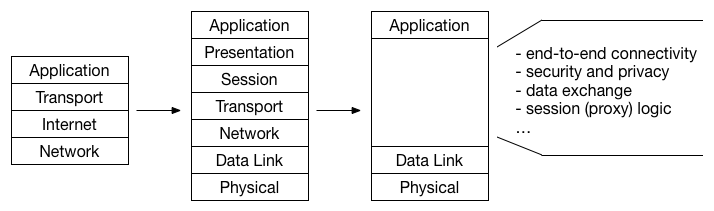
\includegraphics[width=0.8\linewidth]{Figures/tcpstack.png}
	\caption[]{TCP/IP stack}
	\label{fig:TCP/IP stack}
\end{figure}
\par
ICN tries to reallocate the functionality needed to get data from the network into sensible abstractions that better suit today’s applications.
ICN offers a compelling alternative to networking that might help us chip away at the technical debt that has accrued as our dependence on the TCP/IP model grew.
 This is the protocol stack of the new internet paradigm ICN. Fig. \ref{fig:stack}.
 \begin{figure}[h]
	\centering
	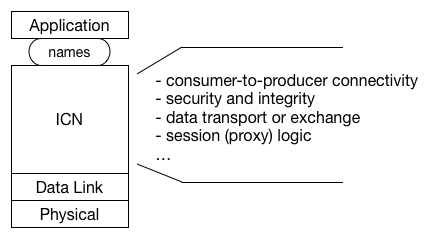
\includegraphics[width=0.8\linewidth]{Figures/stack.png}
	\caption[]{ICN stack}
	\label{fig:stack}
\end{figure}

 
\subsection{IoT Middleware architecture}
The unified IoT architecture, in which the middleware IoT services are proposed for administrative purposes such as towards onboarding devices, device/service discovery and naming. Other functions such as name publishing, discovery, and delivery of the IoT data/services is directly implemented in the ICN network.
The proposed ICN-IoT unified architecture. Fig. 
 \ref{fig:archi}.
 \begin{figure}[h]
	\centering
	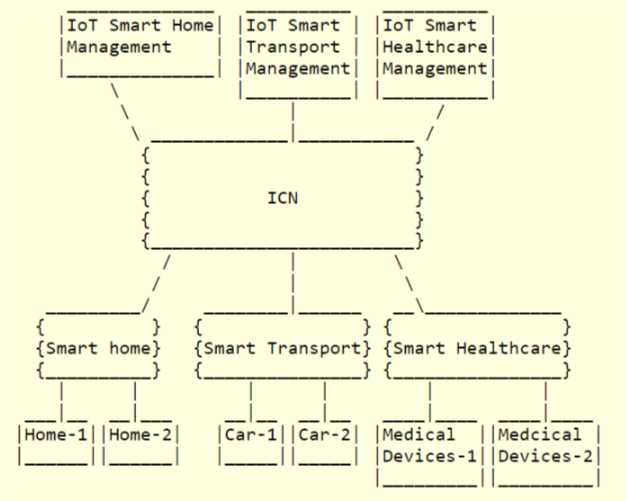
\includegraphics[width=0.8\linewidth]{Figures/archi.png}
	\caption[]{ICN-IoT unified architecture}
	\label{fig:archi}
\end{figure}
\par

The five components of the architecture:
\begin{enumerate}
\item Embedded system
\item Aggregator
\item Local Service Gateway(LSG)
\item ICN-IoT Server
\item Service/Consumer
\end{enumerate}
Here is the middleware Fig. \ref{fig:architecture}.
\begin{figure}[h]
	\centering
	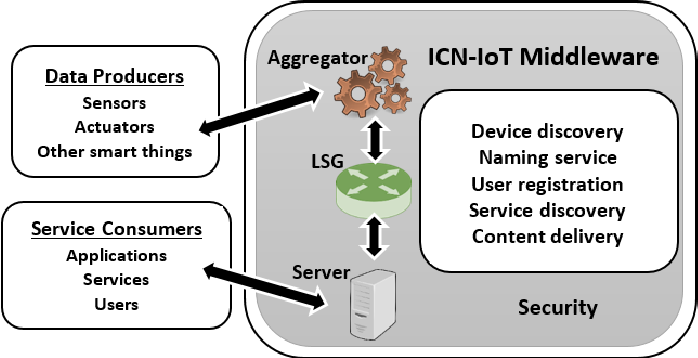
\includegraphics[width=0.8\linewidth]{Figures/Architecture.png}
	\caption[]{Middleware architecture}
	\label{fig:architecture}
\end{figure}
\par
Embedded Systems (ES): The embedded sensor has sensing and actuating functions and may also be able to relay data for other sensors to the Aggregator, through wireless or wired links.
Aggregator: It interconnects various entities in a local IoT network. Aggregators serve the following functionalities: device discovery, service discovery, and name assignment. Aggregators can communication with each other directly or through the local service gateway.\par
Local Service Gateway (LSG): A LSG serves the following functionalities: (1) it is at the administrative boundary, such as, the home or an enterprise, connecting the local IoT system to the rest of the global IoT system, (2) it serves to assign ICN names to local sensors, (3) it enforces data access policies for local IoT devices, and (4) it runs context processing services to generate information specified by application-specific contexts (instead of raw data) to the IoT server.\par
ICN-IoT Server: Within a given IoT service context, the IoT server is a centralized server that maintains subscription memberships and provides the lookup service for subscribers. Unlike legacy IoT servers that are involved in the data path from publishers to subscribers -- raising the concern of its interfaces being a bottleneck -- the IoT server in our architecture is only involved in the control path where publishers and subscribers exchange their names, certificates, and impose other security functions such as access control.\par
Authentication Manager (AM): The authentication manager serves to enable authentication of the embedded devices when they are onboarded in the network and also if their identities need to be validated at the overall system level. The authentication manager may be co-resident with the LSG or the IoT server, but it can also be standalone inside the administrative boundary or outside it.\par
Services/Consumer: These are other application instances interacting with the IoT server to fetch or be notified of anything of interest within the scope of the IoT service.\par






